\documentclass[journal,12pt,twocolumn]{IEEEtran}
\usepackage{setspace}
\usepackage{gensymb}
\singlespacing
\usepackage[cmex10]{amsmath}
\usepackage{amsthm}
\usepackage{mathrsfs}
\usepackage{txfonts}
\usepackage{stfloats}
\usepackage{bm}
\usepackage{cite}
\usepackage{cases}
\usepackage{subfig}
\usepackage{longtable}
\usepackage{multirow}
\usepackage{enumitem}
\usepackage{mathtools}
\usepackage{steinmetz}
\usepackage{tikz}
\usepackage{circuitikz}
\usepackage{verbatim}
\usepackage{tfrupee}
\usepackage[breaklinks=true]{hyperref}
\usepackage{graphicx}
\usepackage{tkz-euclide}
\usetikzlibrary{calc,math}
\usepackage{listings}
\usepackage{color}                                            
\usepackage{array}                                            
\usepackage{longtable}                                        
\usepackage{calc}                                             
\usepackage{multirow}                                         
\usepackage{hhline}                                          
\usepackage{ifthen}                                           
\usepackage{lscape}     
\usepackage{multicol}
\usepackage{chngcntr}
\DeclareMathOperator*{\Res}{Res}
\renewcommand\thesection{\arabic{section}}
\renewcommand\thesubsection{\thesection.\arabic{subsection}}
\renewcommand\thesubsubsection{\thesubsection.\arabic{subsubsection}}
\renewcommand\thesectiondis{\arabic{section}}
\renewcommand\thesubsectiondis{\thesectiondis.\arabic{subsection}}
\renewcommand\thesubsubsectiondis{\thesubsectiondis.\arabic{subsubsection}}
\hyphenation{op-tical net-works semi-conduc-tor}
\def\inputGnumericTable{}                                 %%
\lstset
{
%language=C,
frame=single, 
breaklines=true,
columns=fullflexible
}
\begin{document}
\newcommand{\BEQA}{\begin{eqnarray}}
\newcommand{\EEQA}{\end{eqnarray}}
\newcommand{\define}{\stackrel{\triangle}{=}}
\bibliographystyle{IEEEtran}
\raggedbottom
\setlength{\parindent}{0pt}
\providecommand{\mbf}{\mathbf}
\providecommand{\pr}[1]{\ensuremath{\Pr\left(#1\right)}}
\providecommand{\qfunc}[1]{\ensuremath{Q\left(#1\right)}}
\providecommand{\sbrak}[1]{\ensuremath{{}\left[#1\right]}}
\providecommand{\lsbrak}[1]{\ensuremath{{}\left[#1\right.}}
\providecommand{\rsbrak}[1]{\ensuremath{{}\left.#1\right]}}
\providecommand{\brak}[1]{\ensuremath{\left(#1\right)}}
\providecommand{\lbrak}[1]{\ensuremath{\left(#1\right.}}
\providecommand{\rbrak}[1]{\ensuremath{\left.#1\right)}}
\providecommand{\cbrak}[1]{\ensuremath{\left\{#1\right\}}}
\providecommand{\lcbrak}[1]{\ensuremath{\left\{#1\right.}}
\providecommand{\rcbrak}[1]{\ensuremath{\left.#1\right\}}}
\theoremstyle{remark}
\newtheorem{rem}{Remark}
\newcommand{\sgn}{\mathop{\mathrm{sgn}}}
\providecommand{\abs}[1]{\vert#1\vert}
\providecommand{\res}[1]{\Res\displaylimits_{#1}} 
\providecommand{\norm}[1]{\lVert#1\rVert}
%\providecommand{\norm}[1]{\lVert#1\rVert}
\providecommand{\mtx}[1]{\mathbf{#1}}
\providecommand{\mean}[1]{E[#1]}
\providecommand{\fourier}{\overset{\mathcal{F}}{ \rightleftharpoons}}
%\providecommand{\hilbert}{\overset{\mathcal{H}}{ \rightleftharpoons}}
\providecommand{\system}{\overset{\mathcal{H}}{ \longleftrightarrow}}
%\newcommand{\solution}[2]{\textbf{Solution:}{#1}}
\newcommand{\solution}{\noindent \textbf{Solution: }}
\newcommand{\cosec}{\,\text{cosec}\,}
\providecommand{\dec}[2]{\ensuremath{\overset{#1}{\underset{#2}{\gtrless}}}}
\newcommand{\myvec}[1]{\ensuremath{\begin{pmatrix}#1\end{pmatrix}}}
\newcommand{\mydet}[1]{\ensuremath{\begin{vmatrix}#1\end{vmatrix}}}
\numberwithin{equation}{subsection}
\makeatletter
\@addtoreset{figure}{problem}
\makeatother
\let\StandardTheFigure\thefigure
\let\vec\mathbf
\renewcommand{\thefigure}{\theproblem}
\def\putbox#1#2#3{\makebox[0in][l]{\makebox[#1][l]{}\raisebox{\baselineskip}[0in][0in]{\raisebox{#2}[0in][0in]{#3}}}}
\def\rightbox#1{\makebox[0in][r]{#1}}
\def\centbox#1{\makebox[0in]{#1}}
\def\topbox#1{\raisebox{-\baselineskip}[0in][0in]{#1}}
\def\midbox#1{\raisebox{-0.5\baselineskip}[0in][0in]{#1}}
\vspace{3cm}
\title{AI1103 Assignment-4}
\author{V Rahul - AI20BTECH11030}
\maketitle
\newpage
\bigskip
\renewcommand{\thefigure}{\theenumi}
\renewcommand{\thetable}{\theenumi}


Download all python codes from 
\begin{lstlisting}
    https://github.com/vrahul02/AI1103-Probability-and-Random-Variables/tree/main/Assignment-4/Codes
\end{lstlisting}
%
and latex-tikz codes from 
%
\begin{lstlisting}
    https://github.com/vrahul02/AI1103-Probability-and-Random-Variables/tree/main/Assignment-4/Assignment-4.tex
\end{lstlisting}


\section*{Problem GATE 2021 (ST), Q.15}
A fair die is rolled twice independently. Let X and Y denote the outcomes of the first and second roll, respectively. Then $E(X+Y\:|\:(X-Y)^2=1)$ equals


\section*{Solution}
X and Y are two independent random variables that can take the values 1, 2, 3, 4, 5, 6.
\begin{align}
    \Pr\brak{X=k}=\frac{1}{6}, 1\leq k \leq 6\\
    \Pr\brak{Y=k}=\frac{1}{6}, 1\leq k \leq 6
\end{align}
On using convolution for discrete random variables,\\
$\Pr\brak{X+Y=n}$
\begin{align}
    =&\sum_{k=n-6}^{n-1} \Pr\brak{X=k,Y=n-k}, 1\leq k \leq 6
\end{align}
Since X and Y are independent random variables,
\begin{align}
    =&\sum_{k=n-6}^{n-1} \Pr\brak{X=k}\times\Pr\brak{Y=n-k}, 1\leq k \leq 6\\
    =&\sum_{k=n-6}^{n-1} \frac{1}{6}\times\frac{1}{6}, 1\leq k \leq 6\\
    =&\sum_{k=n-6}^{n-1} \frac{1}{36}, 1\leq k \leq 6\label{0.0.12}
\end{align}
\begin{figure}[htb]
    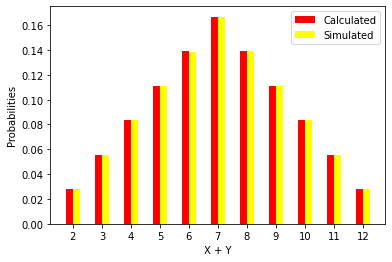
\includegraphics[width=\columnwidth]{Assignment-4(1).png}
    \caption{Plot of PMF for X+Y}
\end{figure}
\newline
$\Pr\brak{X-Y=n}$
\begin{align}
    =&\sum_{k=n+1}^{n+6} \Pr\brak{X=k,Y=k-n}, 1\leq k \leq 6
\end{align}
Since X and Y are independent random variables,
\begin{align}
    =&\sum_{k=n+1}^{n+6} \Pr\brak{X=k}\times\Pr\brak{Y=k-n}, 1\leq k \leq 6\\
    =&\sum_{k=n+1}^{n+6} \frac{1}{6}\times\frac{1}{6}, 1\leq k \leq 6\\
    =&\sum_{k=n+1}^{n+6} \frac{1}{36}, 1\leq k \leq 6\label{0.0.16}
\end{align}
\begin{figure}[htb]
    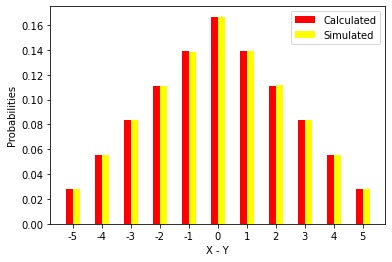
\includegraphics[width=\columnwidth]{Assignment-4(2).png}
    \caption{Plot of PMF for X-Y}
\end{figure}
\begin{align}
    (X-Y)^2=1\\
    X-Y=+1,\:X-Y=-1
\end{align}
$E\brak{X+Y\:|\:(X-Y)^2=1}$
\begin{align}
    =&\sum\:n\times\Pr\brak{X+Y=n\:|\:(X-Y)^2=1}
\end{align}
\begin{align}
    =&\sum\:n\times\frac{\Pr\brak{X+Y=n,(X-Y)^2=1}}{\Pr\brak{(X-Y)^2=1}}
\end{align}
\begin{align}
    \begin{split}
        =\sum\:n\times\frac{\Pr\brak{X+Y=n,(X-Y)=1}}{\Pr\brak{(X-Y)=1}}
        \bigskip\\
        \times\Pr\brak{(X-Y)=1|(X-Y)^2=1}
        \bigskip\\
        +\sum\:n\times\frac{\Pr\brak{X+Y=n,(X-Y)=-1}}{\Pr\brak{(X-Y)=-1}}
        \bigskip\\
        \times\Pr\brak{(X-Y)=1\:|\:(X-Y)^2=1}
    \end{split}
\end{align}
\begin{align}
    \begin{split}
        =\:\frac{\Pr\brak{(X-Y)=1\:|\:(X-Y)^2=1}}{\Pr\brak{(X-Y)=1}}
        \bigskip\\
        \times\sum\:n\times\Pr\brak{X+Y=n,(X-Y)=1}
        \bigskip\\
        +\frac{\Pr\brak{(X-Y)=-1\:|\:(X-Y)^2=1}}{\Pr\brak{(X-Y)=-1}}
        \bigskip\\
        \times\sum\:n\times\Pr\brak{X+Y=n,(X-Y)=-1}\label{0.0.8}
    \end{split}
\end{align}
\newline
Using equations \eqref{0.0.12} and \eqref{0.0.16} in \eqref{0.0.8}\\
We get,\\
$E\brak{X+Y\:|\:(X-Y)^2=1}$
\begin{align}
    =&\:\brak{\frac{\frac{1}{2}}{\frac{5}{36}}}\times\brak{\frac{35}{36}}+\brak{\frac{\frac{1}{2}}{\frac{5}{36}}}\times\brak{\frac{35}{36}}\\
    =&\:7
\end{align}
\end{document}